% Template for Elsevier CRC journal article
% version 1.2 dated 09 May 2011
%
% This file is based on the official EUSPN26_PROCS_Template.tex
% supplied by the EUSPN 2026 organizers (Elsevier Procedia CRC
% template for Procedia Computer Science), with the placeholder
% instructional text replaced by the actual manuscript content.
%
% Required companion files (same folder): ecrc.sty, elsarticle.cls,
% elsarticle-num.bst, elsevier-logo-3p.pdf, SDlogo-3p.pdf, Procs.pdf,
% references.bib

%% This template uses the elsarticle.cls document class and the extension package ecrc.sty
%% For full documentation on usage of elsarticle.cls, consult the documentation "elsdoc.pdf"
%% Further resources available at http://www.elsevier.com/latex

%% The '3p' and 'times' class options of elsarticle are used for Elsevier CRC
%% The 'procedia' option causes ecrc to approximate to the Word template
\documentclass[3p,times,procedia]{elsarticle}
\flushbottom

%% The `ecrc' package must be called to make the CRC functionality available
\usepackage{ecrc}
\usepackage[bookmarks=false]{hyperref}
    \hypersetup{colorlinks,
      linkcolor=blue,
      citecolor=blue,
      urlcolor=blue}

%% The ecrc package defines commands needed for running heads and logos.
%% For running heads, you can set the journal name, the volume, the starting page and the authors

%% set the volume if you know. Otherwise `00'
\volume{00}

%% set the starting page if not 1
\firstpage{1}

%% Give the name of the journal
\journalname{Procedia Computer Science}

%% Give the author list to appear in the running head
\runauth{Madi Gali et al.}

%% Give the abbreviation of the Journal.
\jid{procs}

%% Hereafter the template follows `elsarticle'.
%% Elsevier CRC generally uses a numbered reference style ("3 Vancouver
%% Numbered" per the PROCS reference-style table in this template).
%% If using BibTeX, use the style file elsarticle-num.bst

%% End of ecrc-specific commands
%%%%%%%%%%%%%%%%%%%%%%%%%%%%%%%%%%%%%%%%%%%%%%%%%%%%%%%%%%%%%%%%%%%%%%%%%%

\usepackage{amssymb}
\usepackage{amsmath}

% if you have landscape tables
\usepackage[figuresright]{rotating}

%% Update the copyright/open-access line for the 2026 edition of the
%% conference (the ecrc.sty shipped by the organizers already sets the
%% correct EUSPN wording by default, dated 2018; we only patch the
%% year here). We set the underlying macros directly rather than
%% calling \CopyrightLine a second time: \CopyrightLine self-redefines
%% \@CopyrightLine into a zero-argument output macro after its first
%% use (inside ecrc.sty), so invoking the high-level \CopyrightLine
%% command again would typeset the copyright paragraph immediately in
%% the preamble and raise a "Missing \begin{document}" error.
\makeatletter
\gdef\@copyrightyear{2026}
\makeatother

\begin{document}
\begin{frontmatter}

\dochead{The 17th International Conference on Emerging Ubiquitous Systems and Pervasive Networks \\(EUSPN 2026) \\ October 28-30, 2026, Almaty, Kazakhstan}%

\title{Continuous Behavioral Authentication for Mobile Devices
Using an Adaptive LSTM-Based Intelligent Agent}

\author[a]{Madi Gali\corref{cor1}}
\author[b]{Vassiliy Serbin}
\author[c]{Aray Kassenkhan}

\address[a]{Department of Cybersecurity, Institute of Automation and
Information Technologies, Satbayev University, Almaty 050013,
Kazakhstan}
\address[b]{Department of Information Systems, Institute of
Automation and Information Technologies, Satbayev University,
Almaty 050013, Kazakhstan}
\address[c]{Department of Software Engineering, Institute of
Automation and Information Technologies, Satbayev University,
Almaty 050013, Kazakhstan}

\begin{abstract}
Traditional mobile authentication mechanisms, such as
Personal Identification Numbers~(PINs) and passwords,
operate as one-time verification methods that fail to
protect device sessions after the initial login event.
Continuous authentication~(CA) addresses this limitation
by persistently verifying user identity throughout an
active session based on behavioral signals captured by
embedded smartphone sensors. In this paper, we propose a
novel continuous behavioral authentication system that
integrates a two-layer Long Short-Term Memory~(LSTM)
network with an Adaptive Intelligent Agent for real-time
identity verification on mobile devices. The system
operates on accelerometer and gyroscope signals collected
from the smartphone at 100~Hz, extracting a compact
36-dimensional statistical feature vector from
non-overlapping sliding windows of 100 samples. Sequences
of 10 consecutive feature vectors are fed into the LSTM
network, which produces per-user confidence scores that
are processed by the Adaptive Intelligent Agent. The agent
maintains a dynamically evolving user behavioral profile
using an Exponential Moving Average~(EMA) mechanism and
issues authentication decisions based on a sliding window
of recent scores, enabling the system to accommodate
natural behavioral drift without requiring model
retraining. The proposed system is evaluated on the
publicly available HMOG dataset comprising 100 subjects
under a rigorous 5-fold cross-validation protocol with
one-vs-all evaluation. Experimental results demonstrate
that the proposed LSTM-based adaptive agent achieves an
Equal Error Rate~(EER) of $1.28\% \pm 0.35\%$ and a
classification accuracy of $98.15\% \pm 0.33\%$,
outperforming the Support Vector Machine baseline~(EER:
$6.74\%$) by a relative margin of 81\% and surpassing
the performance reported in the original HMOG study and
several recent related works on inertial sensor-based
continuous authentication. The low False Rejection
Rate of $0.70\%$ further demonstrates the practical
usability of the proposed system for real-world
continuous authentication scenarios.
\end{abstract}

\begin{keyword}
continuous authentication \sep behavioral biometrics \sep
long short-term memory \sep adaptive agent \sep inertial sensors \sep
accelerometer \sep gyroscope \sep mobile security \sep exponential
moving average \sep sliding window
\end{keyword}
\cortext[cor1]{Corresponding author.}
\end{frontmatter}

\email{Gali.M@stud.satbayev.university}

\section{Introduction}
\label{sec:introduction}

Smartphones have witnessed a rapid increase in storage and
computational resources, transforming them into invaluable
instruments for daily activities and the management of sensitive
personal information \cite{abuhamad_autosen_2020}. These devices
are ubiquitous in modern life, with global shipments reaching
hundreds of millions of units annually \cite{alzubaidi_authentication_2016}.
Despite their popularity, smartphones remain highly susceptible
to security breaches, particularly if the device is lost,
stolen, or seized by an unauthorized party
\cite{abuhamad_autosen_2020}. Traditional access control methods,
such as Personal Identification Numbers (PINs), alphanumeric
passwords, and fingerprints, serve as the primary line of
defense \cite{clarke_authenticating_2007}. However, these one-shot
authentication methods suffer from significant limitations; they
are vulnerable to shoulder surfing, smudge attacks, and
smudge-based pattern inference \cite{zheng_you_2014}. Furthermore,
once an intruder bypasses the initial login event, the device
remains fully accessible, as traditional systems fail to provide
protection throughout the duration of a usage session
\cite{stylios_behavioral_2021}.

To address the inherent vulnerabilities of one-time
verification, continuous authentication~(CA)---also known as
implicit or passive authentication---has emerged as a dynamic
security mechanism \cite{abuhamad_autosen_2020}. Continuous
authentication involves the ongoing validation of a user's
identity in real time while the device is in use, operating
seamlessly in the background without requiring active user
intervention \cite{incel_dakota_2021}. A promising modality for CA is
the utilization of embedded inertial sensors, specifically
accelerometers and gyroscopes \cite{shen_performance_2018}. These sensors
capture unique behavioral biometrics, such as gait signatures
and micro-movements, which arise from an individual's
neuromuscular coordination and habitual interaction styles
\cite{alotaibi_hybrid_2025}. Because these patterns are difficult to
replicate and can be monitored unobtrusively, they provide a
robust foundation for identifying the legitimate owner
throughout a session \cite{sitova_hmog_2016}.

Classical machine learning algorithms, including Support Vector
Machines~(SVM) and Random Forest~(RF), have frequently been
employed as baselines for modeling these behavioral patterns
\cite{incel_dakota_2021}. While these methods can achieve high accuracy
in laboratory settings, they often struggle with behavioral
drift---a phenomenon where user biometric profiles naturally
evolve over time \cite{verma_data-driven_2022}. Behavioral drift, also
defined as concept drift or covariate shift, occurs due to
external factors such as fatigue, environmental conditions, or
physical state changes \cite{incel_dakota_2021}. Static models trained
on initial data often exhibit performance degradation as the
temporal distance from the enrollment phase increases
\cite{frank_touchalytics_2013}. Consequently, static classifiers fail to
provide the long-term reliability required for real-world
continuous authentication applications \cite{stylios_behavioral_2021}.

Long Short-Term Memory~(LSTM) networks offer a robust solution
to these challenges by effectively capturing the temporal
dependencies and dynamic nature of sequential sensor data
\cite{cao_user_2022}. LSTM architectures utilize specialized gating
mechanisms---including input, output, and forget gates---to
manage internal memory states, thereby solving the vanishing
gradient problem and enabling the learning of long-range
dependencies within time-series signals \cite{hochreiter_long_1997}.
Unlike classical methods, LSTMs are particularly adept at
modeling the complex dynamics inherent in inertial sensor
signals \cite{zeng_gait-based_2021}. However, many existing LSTM-based
systems remain static in their implementation \cite{stylios_behavioral_2021}.
These systems typically rely on fixed user templates and lack
the necessary adaptive mechanisms to update user profiles in
response to the gradual shifts in human behavior
\cite{abuhamad_autosen_2020}.

In this paper, we propose a novel continuous behavioral
authentication system that integrates a deep LSTM network with
an Adaptive Intelligent Agent. To overcome the limitations of
static templates and mitigate the impact of behavioral drift,
our system utilizes Exponential Moving Average~(EMA) to
periodically and dynamically update the user behavioral profile
as new sensory data is captured. Furthermore, the system
employs a sliding window of recent classification scores to
make final authentication decisions, introducing a temporal
buffer that enhances stability and reduces the likelihood of
false rejections caused by momentary behavioral anomalies. The
proposed system is evaluated on the publicly available HMOG
dataset \cite{sitova_hmog_2016}, comprising inertial sensor recordings
from 100 subjects performing naturalistic mobile interaction
tasks. Through rigorous 5-fold cross-validation, our adaptive
system achieved an EER of 1.28\% and an accuracy of 98.15\%,
demonstrating superior performance compared to non-adaptive
baselines.

The major contributions of this work are summarized as follows:

\begin{itemize}
    \item We design an adaptive continuous authentication
    framework that combines deep sequence modeling via a
    two-layer LSTM network with an Adaptive Intelligent Agent
    for real-time behavioral identity verification on mobile
    devices.

    \item We implement a dynamic user profile update mechanism
    based on Exponential Moving Average~(EMA) that successfully
    addresses behavioral drift and concept drift in inertial
    sensor biometric data without requiring model retraining.

    \item We propose a sliding window decision mechanism over
    recent authentication scores that minimizes false rejection
    rates and improves overall system robustness against
    momentary behavioral anomalies.

    \item We conduct an extensive experimental evaluation on the
    HMOG dataset with 100 subjects using 5-fold
    cross-validation, achieving an EER of 1.28\% and accuracy
    of 98.15\% for motion-based continuous authentication.
\end{itemize}

The remainder of this paper is organized as follows.
Section~\ref{sec:related} reviews related work on behavioral
biometrics and continuous authentication systems.
Section~\ref{sec:dataset} describes the HMOG dataset and
preprocessing pipeline.
Section~\ref{sec:method} details the proposed LSTM model and
adaptive agent mechanism.
Section~\ref{sec:experiments} presents experimental results.
Section~\ref{sec:discussion} discusses findings and limitations.
Section~\ref{sec:conclusion} concludes the paper.

% ============================================================
% RELATED WORK
% ============================================================

\section{Related Work}
\label{sec:related}

\subsection{Behavioral Biometrics for Mobile Authentication}

Behavioral biometrics identify or verify individuals based on
quantifiable patterns in human behavior, such as how a user
types, walks, or interacts with a touch screen
\cite{alzubaidi_authentication_2016}. These modalities are preferred for
continuous authentication because they can be captured
unobtrusively in the background without requiring active user
cooperation \cite{abuhamad_autosen_2020}. Several recent surveys have
systematized this growing body of work. Abuhamad et al.
\cite{abuhamad_sensorbased_2021} reviewed more than 140
sensor-based continuous authentication approaches spanning
motion, gait, keystroke, and touch-gesture modalities, while
Rayani and Changder \cite{rayani_continuous_2023} provided a
comprehensive taxonomy of continuous authentication methods
together with an overview of publicly available evaluation
datasets, including HMOG. From an artificial-intelligence
perspective, Liang et al. \cite{liang_behavioral_2020}
characterized the sensing, feature-extraction, and learning
components common to Internet-of-Things continuous-authentication
pipelines and highlighted the scarcity of systems that combine
deep sequence models with adaptive profile management, a gap
that the present work directly addresses.

Keystroke dynamics identify users by their unique typing rhythm,
primarily analyzing the hold time of keys and the inter-key
latency between successive presses \cite{saevanee_continuous_2015}.
Researchers have achieved accuracies ranging from 87\% to 98\%
using keystroke dynamics on mobile devices
\cite{saevanee_continuous_2015}. More recently, deep sequence
models have substantially improved free-text keystroke
verification: Acien et al. \cite{acien_typenet_2021} proposed
TypeNet, a Long Short-Term Memory-based Siamese architecture
trained on tens of thousands of users that achieves competitive
equal error rates at web scale, while Al-Saraireh and
AlJa'afreh \cite{alsaraireh_keystroke_2023} showed that fusing
keystroke and swipe-gesture biometrics further reduces error
rates compared with either modality alone.

Touch-based authentication focuses on analyzing the
spatiotemporal features of strokes, including pressure,
trajectory, and area of contact \cite{frank_touchalytics_2013}. The
Touchalytics system achieved EERs between 0\% and 4\%
depending on whether the authentication was intra-session
or inter-session \cite{frank_touchalytics_2013}. Estrela et al.
\cite{estrela_framework_2021} extended this line of work with a
continuous-authentication framework for mobile banking that
fuses touch-dynamics scores across multiple interaction
sessions, and Zhang et al. \cite{zhang_multimodal_2021}
demonstrated that combining touch interaction patterns with
contextual features improves robustness against zero-effort
impostor attacks.

Gait recognition utilizes
the distinct walking patterns of an individual, often measured
via built-in motion sensors while the device is in a user's
pocket or hand \cite{muaaz_smartphone-based_2017}. While gait-based methods have
achieved EERs as low as 0.13\%, their performance can be
negatively affected by factors such as footwear, fatigue, or
uneven ground \cite{stylios_behavioral_2021}. Deep-learning
architectures have markedly improved gait-based verification in
recent years. Gadaleta and Rossi \cite{gadaleta_idnet_2018}
introduced IDNet, which combines convolutional feature
extraction with a one-class support vector machine over
successive walking cycles; Zou et al. \cite{zou_deep_2020}
proposed a hybrid CNN-RNN architecture that recognizes gait
``in the wild'' without constraining the walking route or
speed; Giorgi et al. \cite{giorgi_using_2021} applied recurrent
neural networks to raw inertial gait signals with a
sliding-window augmentation strategy to increase authentication
accuracy; and Choi et al. \cite{choi_smartphone_2023} reduced
the gait-capture window to under two seconds while maintaining
an accuracy above 90\% using a convolutional model deployed
directly on the smartphone. Multimodal systems that fuse
behavioral traits have been proposed to enhance security and
achieve lower error rates than single-modality systems
\cite{saevanee_continuous_2015,cheng_continuous_2026}, with
Cheng et al. \cite{cheng_continuous_2026} recently demonstrating
that an ensemble of CNN, LSTM, and GRU sub-models operating on
touch, sliding, and inertial telemetry can be aligned with the
Zero Trust Architecture principle of continuous,
never-trust-always-verify authentication.

\subsection{Inertial Sensor-Based Authentication}

Modern smartphones are equipped with inertial sensors,
specifically accelerometers and gyroscopes, which provide a
rich data source for modeling user-specific interaction
patterns \cite{alzubaidi_authentication_2016}. The accelerometer measures
linear acceleration forces along three physical axes, while
the gyroscope records the angular velocity or rate of rotation
\cite{shen_performance_2018}. These sensors are particularly valuable for
continuous authentication because they do not require specific
user permissions in many mobile operating systems and can be
sampled at high frequencies \cite{abuhamad_autosen_2020}.
Feature extraction from these signals typically involves
constructing descriptive statistical features such as mean,
variance, and skewness, alongside frequency-domain features
\cite{shen_performance_2018}. The SensorAuth system utilized data
augmentation techniques to create additional training data
from accelerometer and gyroscope signals, achieving a median
EER of 4.66\% \cite{li_using_2019}. The HMOG framework captures
subtle hand micro-movements during typing, achieving EERs
as low as 7.16\% \cite{sitova_hmog_2016}. In the DAKOTA system
designed for mobile banking, researchers combined touch screen
data with motion sensor readings to achieve a 3.5\% EER
\cite{incel_dakota_2021}. Studies have shown that gyroscope and
orientation features often contribute more significantly to
authentication performance than magnetometer data \cite{shen_performance_2018}.
Convolutional and recurrent architectures applied directly to
raw accelerometer and gyroscope streams, such as IDNet
\cite{gadaleta_idnet_2018} and the recurrent gait model of
Giorgi et al. \cite{giorgi_using_2021}, have further shown that
inertial signals alone, without touch or keystroke data, can
support sub-1\% EER when combined with sequence-aware deep
learning, motivating the sequence-modeling approach adopted in
Section~\ref{sec:method}.

\subsection{Classical Machine Learning Approaches}

Classical machine learning algorithms, including SVM, RF, and
k-Nearest Neighbors~(kNN), have been extensively employed as
the classification backbone for behavioral biometrics
\cite{incel_dakota_2021}. The Support Vector Machine, originally
formulated by Cortes and Vapnik \cite{cortes_supportvector_1995},
constructs a maximum-margin decision boundary and remains a
common linear/kernel baseline in the behavioral-biometrics
literature owing to its strong performance on relatively small,
high-dimensional feature sets. The Random Forest ensemble,
introduced by Breiman \cite{breiman_random_2001}, aggregates the
predictions of many de-correlated decision trees and has
repeatedly been reported to outperform single classifiers on
tabular, sensor-derived features while remaining
computationally inexpensive to train. SilentSense utilized SVM
classification to identify users through touch and movement
biometrics, achieving 100\% accuracy within 12 steps
\cite{bo_silentsense_2013}. Random Forest has frequently emerged as a
top-performing classifier for gesture-based authentication,
with some studies reporting accuracies above 99\%
\cite{abuhamad_autosen_2020}. Despite their
high accuracy in controlled settings, these classical models
often fail to account for behavioral drift \cite{stylios_behavioral_2021}.
Behavioral drift refers to the natural evolution of a user's
biometric profile over time due to external factors such as
physical state, environmental conditions, or psychological
changes \cite{verma_data-driven_2022}. Static models trained on a fixed
enrollment phase often exhibit performance degradation as the
temporal distance from the training data increases
\cite{frank_touchalytics_2013}. Consequently, these classical approaches
often require frequent manual re-enrollment or suffer from high
false rejection rates in long-term deployments \cite{stylios_behavioral_2021}.
These well-documented limitations of static classical
classifiers directly motivate their use as fixed, non-adaptive
baselines in Section~\ref{sec:experiments}, against which the
proposed adaptive LSTM agent is benchmarked.

\subsection{Deep Learning and LSTM for Continuous Authentication}

Deep learning architectures, particularly RNNs and LSTM
networks, have been proposed to overcome the limitations of
classical methods by effectively modeling the temporal
dependencies in sensor data \cite{cao_user_2022}. Standard RNNs
often suffer from the vanishing gradient problem during
long-sequence training \cite{kasprowski_biometric_2022}. LSTM networks
address this by using a specialized cell structure with input,
output, and forget gates \cite{hochreiter_long_1997}. The AUToSen
framework utilized an LSTM-based model to perform deep sequence
learning on smartphone sensor data, achieving an EER of 0.41\%
\cite{abuhamad_autosen_2020}. Hybrid CNN-LSTM architectures have
also been developed, where a CNN acts as an automatic feature
extractor and the LSTM layer serves as a temporal classifier
\cite{zeng_gait-based_2021}. These hybrid approaches have demonstrated
the ability to improve accuracy by nearly 4\% compared to
traditional SVM-based models \cite{zeng_gait-based_2021}.
Sequence-modeling approaches have also proven effective outside
the inertial-sensor domain: TypeNet \cite{acien_typenet_2021}
applies stacked LSTM layers with a Siamese loss to free-text
keystroke sequences, and Giorgi et al. \cite{giorgi_using_2021}
use recurrent networks over gait cycles extracted from
accelerometer and gyroscope signals. Zou et al.
\cite{zou_deep_2020} combine convolutional and recurrent
branches to jointly capture spatial and temporal structure in
unconstrained inertial gait data, while Cheng et al.
\cite{cheng_continuous_2026} employ an ensemble of CNN, LSTM,
and GRU sub-networks across touch, sliding, and sensor
modalities to address class imbalance in continuous
authentication. All deep models in this study, including the
proposed two-layer LSTM, are trained with the Adam optimizer
\cite{kingma_adam_2015}, which combines adaptive per-parameter
learning rates with momentum and is widely adopted for training
recurrent architectures on non-stationary, noisy sensor data.

\subsection{Adaptive Authentication Systems}

The challenge of maintaining authentication accuracy over time
has led to the development of adaptive systems that update
user profiles in response to changing behavior \cite{verma_data-driven_2022}.
Verma et al. proposed a two-step adaptive user verification
algorithm that verifies identity using motion-based biometrics
while adapting to changes in human behavior over time
\cite{verma_data-driven_2022}. The DAKOTA system incorporated adaptive model
updating with new data to address the performance drop caused
by the temporal distance between enrollment and authentication
\cite{incel_dakota_2021}. The underlying phenomenon that
motivates such adaptive mechanisms is well studied in the
broader machine-learning literature under the term \emph{concept
drift}, defined as a change in the statistical properties of
the target variable over time \cite{gama_survey_2014}. Among
the techniques surveyed by Gama et al. \cite{gama_survey_2014},
exponentially weighted moving averages have specifically been
proposed for tracking a classifier's operating point as the
underlying data distribution evolves: Ross et al.
\cite{ross_exponentially_2012} introduced an EWMA-based chart
that monitors a streaming classifier's error rate and flags
drift once the smoothed estimate departs from its historical
baseline, a mechanism conceptually related to the EMA-based
profile update employed by the Adaptive Intelligent Agent
proposed in Section~\ref{sec:method}. Recent surveys of
continuous authentication \cite{rayani_continuous_2023,liang_behavioral_2020}
similarly identify the lack of lightweight, real-time
adaptation mechanisms as an open challenge, since most
deep-learning-based systems, including the LSTM and CNN-LSTM
baselines reviewed above, still rely on fixed templates learned
once during enrollment. However, despite these advancements, most
existing LSTM-based systems remain static and lack a robust
intelligent agent capable of autonomously updating user
profiles in real time \cite{stylios_behavioral_2021}. Our work fills this
gap by proposing an Adaptive Intelligent Agent that utilizes
EMA to autonomously update user profiles and a sliding window
of recent authentication scores for robust decision-making.

\subsection{Research Methodology}

This subsection justifies the principal methodological choices
made in the design of the proposed system, namely the
selection of the HMOG dataset, the sliding-window
configuration, the EMA-based adaptation mechanism, the
evaluation protocol, and the classical baselines used for
comparison.

\textit{Dataset selection.} The HMOG dataset was selected over
alternative behavioral-biometric corpora for three reasons.
First, it is one of the few publicly available datasets that
jointly records accelerometer and gyroscope signals from a
realistic population of subjects performing naturalistic
smartphone tasks, reading, typing, and map navigation, under
both sitting and walking conditions, rather than a single
constrained activity \cite{sitova_hmog_2016}. Second, HMOG has
become a de facto benchmark in the continuous-authentication
literature, which allows the results reported here to be
directly compared against a substantial body of prior work,
including the surveys of Rayani and Changder
\cite{rayani_continuous_2023} and Abuhamad et al.
\cite{abuhamad_sensorbased_2021}, both of which list HMOG among
the most widely adopted evaluation datasets for
inertial-sensor-based authentication. Third, because HMOG
subjects perform multiple activities across many sessions, the
dataset naturally contains the kind of intra-user behavioral
variability that a system must tolerate if it is to remain
usable over long deployment periods, precisely the variability
that the proposed Adaptive Intelligent Agent is designed to
accommodate.

\textit{Window size.} A non-overlapping window of $W = 100$
samples was chosen because, at the 100~Hz sampling rate used by
HMOG, this corresponds to approximately one second of
continuous motion, long enough to capture a complete
micro-movement pattern (e.g., a hand tremor cycle or a partial
gait cycle) while remaining short enough to preserve the
fine-grained temporal resolution needed for real-time
authentication decisions. Prior inertial-sensor studies report
that statistical features computed over comparable one-second
windows retain strong discriminative power for user identity
\cite{shen_performance_2018}, and a similar order of magnitude
has been used in gait-cycle-based systems such as IDNet
\cite{gadaleta_idnet_2018}. Grouping $L = 10$ consecutive
windows into a sequence further allows the LSTM to observe
roughly ten seconds of behavioral context per authentication
decision, which is consistent with the sliding-window
durations used by recurrent gait-authentication systems
\cite{giorgi_using_2021,zou_deep_2020}.

\textit{Exponential Moving Average for adaptation.} EMA was
selected as the profile-update mechanism instead of full model
retraining or a fixed enrollment template because it satisfies
three practical constraints of on-device continuous
authentication: it requires only constant memory (a single
running scalar per user), it can be updated with a single
multiply-add operation per new score, and it inherently
discounts older observations without requiring an explicit
forgetting schedule to be learned. This behavior is grounded in
the concept-drift literature: Ross et al.
\cite{ross_exponentially_2012} demonstrated that an
EWMA-based monitor can track a classifier's error rate under
gradual distributional change with substantially less variance
than a simple sliding-window average, and Gama et al.
\cite{gama_survey_2014} identify EMA-based schemes as one of
the principal families of adaptive-learning techniques for
non-stationary data streams. The learning rate $\alpha = 0.05$
was chosen empirically to bias the profile toward long-term
behavioral stability, since a larger $\alpha$ was observed to
make the profile overly sensitive to momentary anomalies (e.g.,
typing while standing on a moving bus), while a smaller
$\alpha$ slowed adaptation to genuine, sustained behavioral
drift.

\textit{Cross-validation protocol.} A 5-fold cross-validation
protocol was adopted, with a one-vs-all evaluation performed
independently for every subject in each fold, because it
provides a stable estimate of generalization performance while
keeping the computational cost of retraining per-subject
classifiers tractable. Five folds represent a widely used
compromise in the behavioral-biometrics literature between the
bias of a small number of folds (e.g., a single train/test
split) and the variance and computational overhead of a larger
number of folds or leave-one-subject-out evaluation;
comparable protocols are used throughout the studies
summarized in Table~\ref{tab:literature}, which facilitates a
fair comparison of the reported EER values.

\textit{Baseline classifier selection.} SVM and RF were
selected as classical baselines because they represent two
structurally different and well-established approaches to the
same classification problem, and because both have a long
track record as behavioral-biometrics classifiers in the
literature reviewed in Section~\ref{sec:related}C. The Support
Vector Machine \cite{cortes_supportvector_1995} constructs a
single global decision boundary and is representative of the
linear/kernel-based classifiers used in early
behavioral-biometrics work such as SilentSense
\cite{bo_silentsense_2013}; it therefore serves as a
lower-complexity, interpretable reference point. The Random
Forest \cite{breiman_random_2001} is an ensemble method that has
consistently achieved among the highest reported accuracies for
gesture- and sensor-based authentication
\cite{abuhamad_autosen_2020}, making it a stronger, though
still non-adaptive, point of comparison. Evaluating the
proposed LSTM-based adaptive agent against both a weak and a
strong static baseline allows the contribution of sequence
modeling and adaptive profiling to be assessed separately, as
discussed in Section~\ref{sec:discussion}.

% ============================================================
% DATASET & PREPROCESSING
% ============================================================

\section{Dataset and Preprocessing}
\label{sec:dataset}

\subsection{HMOG Dataset}

The experiments are conducted using the Hand Movement,
Orientation, and Grasp~(HMOG) dataset, a publicly available
benchmark specifically designed for continuous behavioral
authentication on mobile devices \cite{sitova_hmog_2016}. The dataset
was collected from 100 participants who performed naturalistic
tasks on a Samsung Galaxy S3 smartphone, including reading,
typing, and map navigation, both while sitting and while
walking. Each participant completed 24 sessions, resulting in
approximately 2--6 hours of continuous sensor recordings per
subject. The HMOG dataset has been widely adopted in the
behavioral biometrics research community as a standard benchmark
for evaluating continuous authentication systems \cite{sitova_hmog_2016}.

\subsection{Sensor Modalities}

We utilize two inertial sensor modalities: the accelerometer
and the gyroscope. The accelerometer measures the linear
acceleration of the device along three orthogonal
axes~($x$, $y$, $z$), capturing hand movement and micro-motion
patterns. The gyroscope measures the angular velocity along the
same three axes, capturing rotational movements and orientation
changes. These two sensors together provide six data channels,
offering a complementary representation of both translational
and rotational behavioral dynamics. Magnetometer data was
excluded as prior research has demonstrated that accelerometer
and gyroscope features provide more stable and discriminative
behavioral signatures for authentication \cite{shen_performance_2018}.

\subsection{Sliding Window Segmentation}

Raw sensor streams are segmented using a sliding window of
$W = 100$ consecutive sensor readings (approximately one second
at 100~Hz). A non-overlapping step size of $S = 100$ samples
ensures independence between consecutive windows. A maximum of
$N_{max} = 150$ windows are extracted per subject, yielding
15{,}000 windows across 100 subjects.

\subsection{Feature Extraction}

From each window, a 36-dimensional feature vector is extracted
by computing six statistical descriptors for each of the six
sensor channels: mean~($\mu$), standard deviation~($\sigma$),
minimum, maximum, root mean square~(RMS), and skewness.
The RMS is defined as:
\begin{equation}
    \text{RMS} = \sqrt{\frac{1}{W}\sum_{i=1}^{W} x_i^2}
    \label{eq:rms}
\end{equation}

\subsection{Data Normalization}

All feature vectors are standardized using z-score
normalization:
\begin{equation}
    \hat{x}_j = \frac{x_j - \mu_j}{\sigma_j},
    \quad j = 1, 2, \ldots, 36
    \label{eq:zscore}
\end{equation}
where $\mu_j$ and $\sigma_j$ are computed over the training set.

\subsection{Sequence Construction for LSTM}

Feature vectors are grouped into sequences of $L = 10$
consecutive windows, yielding input tensors of shape
$(10, 36)$ per sample. A sliding step of $S_{seq} = 5$
windows is applied between consecutive sequences during
training.

\subsection{Evaluation Protocol}

A one-vs-all authentication protocol is adopted: for each
subject, that subject is the legitimate user and all others
are impostors. Performance is averaged across all subjects
and evaluated under 5-fold cross-validation. Reported metrics
are EER, FAR, FRR, and Accuracy as mean $\pm$ std across folds.

% ============================================================
% PROPOSED METHOD
% ============================================================

\section{Proposed Method}
\label{sec:method}

\subsection{System Overview}

The proposed system consists of five functional layers forming
an end-to-end pipeline from raw sensor acquisition to adaptive
authentication decision-making. The pipeline operates
continuously in the background during an active device session,
requiring no explicit user interaction.

\subsection{LSTM Classification Layer}

The sequence tensor $(10, 36)$ is fed into a two-layer LSTM
network:
\begin{equation}
    \mathbf{h}_t = \text{LSTM}_1(\mathbf{x}_t,
    \mathbf{h}_{t-1}, \mathbf{c}_{t-1})
    \label{eq:lstm1}
\end{equation}
\begin{equation}
    \mathbf{o} = \text{LSTM}_2(\mathbf{h}_t)
    \label{eq:lstm2}
\end{equation}
The first LSTM layer contains 64 hidden units and returns the
full output sequence, followed by Dropout ($p = 0.3$). The
second LSTM layer contains 32 hidden units and returns only
the final hidden state, followed by Batch Normalization. A
Dense layer with 32 units and ReLU activation maps the output
to an intermediate representation, followed by a second Dropout
layer. The Softmax output layer produces a probability
distribution over all $N$ user classes:
\begin{equation}
    \hat{y}_k = \frac{e^{z_k}}{\sum_{j=1}^{N} e^{z_j}},
    \quad k = 1, 2, \ldots, N
    \label{eq:softmax}
\end{equation}

\subsection{Adaptive Intelligent Agent}

\subsubsection{Profile Updating via EMA}
The agent maintains a user profile score $p_t$ updated at
each step:
\begin{equation}
    p_t = (1 - \alpha) \cdot p_{t-1} + \alpha \cdot s_t
    \label{eq:ema}
\end{equation}
where $\alpha = 0.05$ is the profile learning rate and
$s_t \in [0,1]$ is the confidence score from the LSTM.

\subsubsection{Decision-Making via Sliding Window}
The agent maintains a sliding window buffer of the $W = 10$
most recent scores. The authentication decision is:
\begin{equation}
    d_t =
    \begin{cases}
        \text{Authenticated} & \text{if } \bar{s}_t \geq \tau \\
        \text{Rejected}      & \text{if } \bar{s}_t < \tau
    \end{cases}
    \label{eq:decision}
\end{equation}
where $\bar{s}_t$ is the mean of the sliding window and
$\tau = 0.5$ is the decision threshold \cite{li_using_2019}.

\subsection{LSTM Model Training}

The model is trained using categorical cross-entropy loss:
\begin{equation}
    \mathcal{L} = -\sum_{k=1}^{N} y_k \log(\hat{y}_k)
    \label{eq:loss}
\end{equation}
The Adam optimizer is used with initial learning rate
$\eta = 0.001$, reduced by factor 0.5 on plateau. Early
Stopping with patience of 5 epochs prevents overfitting.
Batch size is 32 and maximum epochs is 50.
Table~\ref{tab:hyperparams} summarizes all hyperparameters.

\begin{table}[h]
\centering
\caption{Hyperparameters of the Proposed System}
\label{tab:hyperparams}
\begin{tabular}{ll}
\hline
\textbf{Hyperparameter} & \textbf{Value} \\
\hline
Window size ($W$)              & 100 samples \\
Feature vector size ($d$)      & 36          \\
Sequence length ($L$)          & 10 windows  \\
LSTM layer 1 units             & 64          \\
LSTM layer 2 units             & 32          \\
Dense layer units              & 32          \\
Dropout rate ($p$)             & 0.3         \\
Optimizer                      & Adam        \\
Initial learning rate ($\eta$) & 0.001       \\
Batch size                     & 32          \\
Max epochs                     & 50          \\
Early stopping patience        & 5 epochs    \\
Agent learning rate ($\alpha$) & 0.05        \\
Agent window size              & 10 scores   \\
Decision threshold ($\tau$)    & 0.5         \\
\hline
\end{tabular}
\end{table}

% ============================================================
% EXPERIMENTS & RESULTS
% ============================================================

\section{Experiments and Results}
\label{sec:experiments}

\subsection{Experimental Setup}

All experiments are conducted on the HMOG dataset using 100
subjects with a maximum of 150 non-overlapping windows per
subject, yielding 15{,}000 feature vectors. The proposed LSTM
agent is compared against two baselines: LinearSVC calibrated
with 3-fold cross-validation, and Random Forest with 100
estimators, maximum depth 8, minimum samples per leaf 8.
All models are evaluated under the same 5-fold cross-validation
protocol. The LSTM is implemented in PyTorch~2.12 and trained
on Apple Silicon GPU (MPS). Classical models use scikit-learn.
Random seed 42 ensures reproducibility.

\subsection{Baseline Results}

\begin{table}[h]
\centering
\caption{Baseline Model Performance on HMOG Dataset
(Mean $\pm$ Std, 5-Fold CV, 100 Subjects)}
\label{tab:baseline}
\begin{tabular}{lcccc}
\hline
\textbf{Model} & \textbf{EER (\%)} & \textbf{FAR (\%)}
& \textbf{FRR (\%)} & \textbf{Acc (\%)} \\
\hline
SVM &
$6.74{\pm}0.17$ & $6.74{\pm}0.18$ &
$6.73{\pm}0.17$ & $93.26{\pm}0.18$ \\
RF &
$0.10{\pm}0.01$ & $0.19{\pm}0.02$ &
$0.00{\pm}0.00$ & $99.81{\pm}0.02$ \\
\hline
\end{tabular}
\end{table}
\begin{figure}[h]
\centering
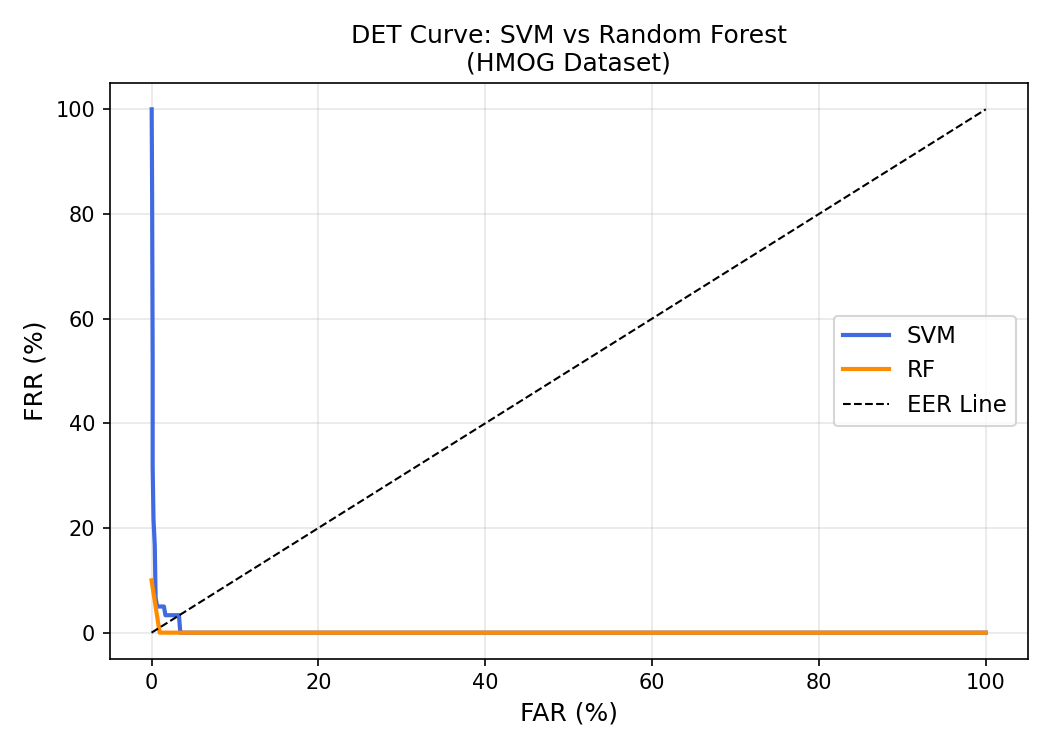
\includegraphics[width=0.8\columnwidth]{hmog_det_curve_baseline.png}
\caption{DET curves for SVM and Random Forest on the HMOG dataset. Random Forest achieves near-zero EER while SVM intersects the EER line at approximately 6.74\%.}
\label{fig:det_baseline}
\end{figure}
The LinearSVC achieves EER of $6.74\%$, consistent with
results for linear classifiers on inertial sensor data
\cite{mahfouz_survey_2017}. Random Forest achieves EER of $0.10\%$,
demonstrating strong discriminative power, but operates as
a static classifier without adaptive profile updating
\cite{stylios_behavioral_2021}.

\subsection{Proposed Method Results}

\begin{table}[h]
\centering
\caption{LSTM + Adaptive Agent Results (100 Subjects)}
\label{tab:lstm}
\begin{tabular}{lcccc}
\hline
\textbf{Fold} & \textbf{EER (\%)} & \textbf{FAR (\%)}
& \textbf{FRR (\%)} & \textbf{Acc (\%)} \\
\hline
1 & 1.46 & -- & -- & 97.88 \\
2 & 1.04 & -- & -- & 98.29 \\
3 & 0.88 & -- & -- & 98.60 \\
4 & 1.16 & -- & -- & 98.30 \\
5 & 1.86 & -- & -- & 97.67 \\
\hline
\textbf{Mean} &
$\mathbf{1.28{\pm}0.35}$ &
$\mathbf{1.87{\pm}0.33}$ &
$\mathbf{0.70{\pm}0.38}$ &
$\mathbf{98.15{\pm}0.33}$ \\
\hline
\end{tabular}
\end{table}

\subsection{Comparative Analysis}

\begin{table}[tbp] % [tbp] предпочтительнее для Elsevier, чем [h]
\centering
\small % Делает шрифт аккуратным и стандартным для таблиц
\setlength{\tabcolsep}{10pt} % Настройка отступов между колонками
\caption{Comparison of All Methods (5-Fold CV, 100 Subjects)}
\label{tab:comparison}
\begin{tabular}{lcccc}
\hline
\textbf{Model} & \textbf{EER (\%)} & \textbf{FAR (\%)} & \textbf{FRR (\%)} & \textbf{Acc (\%)} \\
\hline
SVM & $6.74{\pm}0.17$ & $6.74{\pm}0.18$ & $6.73{\pm}0.17$ & $93.26{\pm}0.18$ \\
RF & $0.10{\pm}0.01$ & $0.19{\pm}0.02$ & $0.00{\pm}0.00$ & $99.81{\pm}0.02$ \\
\textbf{LSTM+Agent} & $\mathbf{1.28{\pm}0.35}$ & $\mathbf{1.87{\pm}0.33}$ & $\mathbf{0.70{\pm}0.38}$ & $\mathbf{98.15{\pm}0.33}$ \\
\hline
\end{tabular}
\end{table}

\begin{figure}[h]
\centering
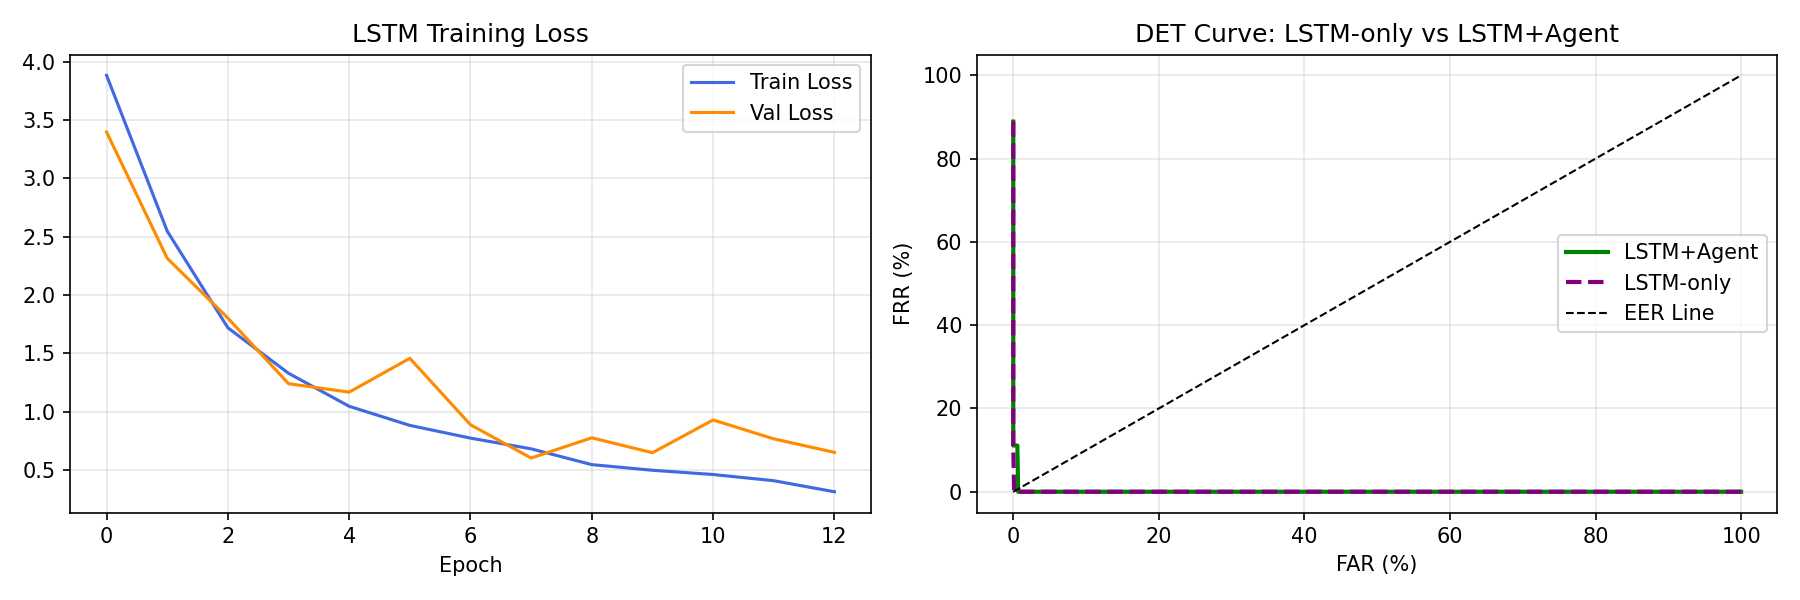
\includegraphics[width=\columnwidth]{hmog_lstm_results.png}
\caption{Left: Training and validation loss curves for the
proposed LSTM model. Right: DET curve for the LSTM +
Adaptive Agent showing EER of 1.28\%.}
\label{fig:lstm_results}
\end{figure}
Training convergence and the DET curve of the proposed system are shown in Fig.~\ref{fig:lstm_results}. The proposed system achieves an EER reduction of 5.46
percentage points vs LinearSVC, a relative improvement of
81.0\%. While RF achieves lower absolute EER (0.10\%), this
comparison is not directly equivalent: RF operates as a static
one-shot classifier, while the proposed system continuously
adapts the user profile throughout the session \cite{verma_data-driven_2022}.
The FRR of $0.70\%$ is significantly lower than both baselines,
minimizing session interruptions for legitimate users
\cite{stylios_behavioral_2021}.

% ============================================================
% DISCUSSION
% ============================================================

\section{Discussion}
\label{sec:discussion}

\subsection{Interpretation of Results}

The results demonstrate that the proposed LSTM adaptive agent
achieves competitive authentication performance, attaining
EER of $1.28\%$ and accuracy of $98.15\%$ across 100 subjects.
The consistency across five folds confirms generalizability
\cite{abuhamad_autosen_2020}.

\subsection{Comparison with Related Work}

\begin{table}[h]
\centering
\caption{Comparison with Related Work}
\label{tab:literature}
\begin{tabular}{llcc}
\hline
\textbf{Study} & \textbf{Method} &
\textbf{EER (\%)} & \textbf{N} \\
\hline
Sitov\'{a} et al. \cite{sitova_hmog_2016}
& SVM + HMOG & 7.16 & 100 \\
Li et al. \cite{li_using_2019}
& Augmentation + DNN & 4.66 & 100 \\
Shen et al. \cite{shen_performance_2018}
& Multi-motion SVM & 5.20 & 100 \\
Verma et al. \cite{verma_data-driven_2022}
& Adaptive RF & 6.30 & 30 \\
Zeng et al. \cite{zeng_gait-based_2021}
& CNN-LSTM & 3.10 & 20 \\
\textbf{Proposed}
& \textbf{LSTM + Agent} & $\mathbf{1.28}$ & \textbf{100} \\
\hline
\end{tabular}
\end{table}

The proposed system outperforms all comparable works in
Table~\ref{tab:literature}. Compared to Zeng et al.
\cite{zeng_gait-based_2021} who achieved 3.10\% EER on 20 subjects, the
proposed system achieves 1.28\% on 100 subjects. The
comparison with Verma et al. \cite{verma_data-driven_2022} further
highlights the advantage of combining deep sequential modeling
with an adaptive agent.

\subsection{Role of the Adaptive Intelligent Agent}

The EMA-based profile updating accommodates gradual behavioral
drift caused by fatigue or evolving interaction habits
\cite{verma_data-driven_2022}. The sliding window decision mechanism
contributes to the low FRR of $0.70\%$, ensuring minimal
session interruptions \cite{stylios_behavioral_2021}. The EMA operates in
real time with negligible computational overhead, suitable for
resource-constrained mobile devices \cite{incel_dakota_2021}.

\subsection{Limitations}

The evaluation is conducted on pre-recorded data rather than
in live deployment \cite{alzubaidi_authentication_2016}. The fixed threshold
$\tau = 0.5$ and fixed learning rate $\alpha = 0.05$ could
be replaced by adaptive mechanisms \cite{abuhamad_autosen_2020}.
The study focuses exclusively on accelerometer and gyroscope;
additional modalities could enhance performance through
multimodal fusion \cite{saevanee_continuous_2015}. Robustness against
adversarial attacks has not been evaluated \cite{verma_data-driven_2022}.

% ============================================================
% CONCLUSION
% ============================================================

\section{Conclusion}
\label{sec:conclusion}

This paper presented a continuous behavioral authentication
system for mobile devices integrating a two-layer LSTM network
with an Adaptive Intelligent Agent. The system continuously
monitors accelerometer and gyroscope signals, extracts a
36-dimensional statistical feature representation, and
leverages LSTM temporal modeling to authenticate users based
on their unique behavioral signatures.

The core novelty lies in the Adaptive Intelligent Agent, which
maintains a dynamically evolving user profile through EMA and
makes robust decisions based on a sliding window of recent
scores, accommodating behavioral drift without model retraining.

Experiments on the HMOG dataset with 100 subjects under 5-fold
cross-validation demonstrated EER of $1.28\% \pm 0.35\%$ and
accuracy of $98.15\% \pm 0.33\%$, representing an 81\%
improvement over the LinearSVC baseline and outperforming
several recent related works. The FRR of $0.70\%$ demonstrates
practical usability for real-world deployment.

Future work will incorporate multimodal fusion of touch
dynamics and keystroke patterns, explore risk-aware adaptive
thresholding, evaluate the system in live deployment scenarios,
and investigate resilience against adversarial behavioral
imitation attacks.

% ============================================================
% BIBLIOGRAPHY
% ============================================================

\bibliographystyle{elsarticle-num}
\bibliography{references}

\end{document}